\chapter{Methodology}
%explain tokens vs. words

Experiments were run on each of three languages\textemdash~Arabic, English, and Korean. Corpus data for Arabic was obtained from the Arabic Treebank: Part 1 v 3.0\cite{maamouri05}, consisting of 165419 tokens of Modern Standard Arabic, where tokens include full words, clitics, and punctuation. Corpus data for English was obtained from a subset of the Open American National Corpus (OANC)\cite{oanc}, consisting of 100165 tokens. Corpus data for Korean was obtained from the data packaged with the KLEX morphological analyzer\cite{han04}, itself a subset of the Korean Treebank, consisting of 41024 tokens. In each case, all data was converted into UTF-8 encoding, with token boundary indices measured in Unicode codepoints. English token boundaries were available in the OANC data in this format, while answer keys for Arabic and Korean were calculated by matching up sequential tokens in part-of-speech tagging files with their locations in the unprocessed plain text, and stored as lists of pairs of starting and ending indices for each token.

\section{Morphological Tokenization}
The simplest dictionary-based tokenization algorithm calculates all possible substrings of the input. Each substring is then checked against the dictionary and, if found, is added to the lattice of possible tokens. In order to reduce the incidence of unknown tokens (particularly important in languages, such as Turkish, with extensive productive morphology, in which most tokens will not appear in a standard dictionary) and reduce the size of the lexicon that needs to be stored, the simple dictionary can be replace by a morphological analyzer to determine whether a given string is or is not a token.

This naïve approach to lattice generation is, however, highly inefficient; given that there are $n-m+1$ substrings of length $m$ in any string of length $n$, and we must check for tokens of all possible lengths (of which there are $n$), the algorithm requires $\sum_{m=1}^{n}(n-m+1)=\frac{1}{2}n(n+1)$ or O$(n^{2})$ time to produce all possible substrings, times a language-specific function $w(m)$ representing the time required to accept or reject a string of length $m$ to produce the lattice of possible tokens. If $w(m)$ is approximately linear (i.e., the amount of time it takes to accept or reject a possible token is, on average, proportional to the length of the token), this results in $\sum_{m=1}^{n}m(n-m+1)=\frac{1}{6}n(n+1)(n+2)$ or O$(n^{3})$ time required to produce all possible tokenizations of a given input. In practice, however, while specific tokens may be unbounded in length, the highly non-random morphological structure of human languages means that most non-tokens will be rejected early since the probability of any randomly selected substring being a valid prefix of the language is inversely related to length. As a result, for long inputs, $w(m)$ is well approximated by a language-specific constant factor $k_w$ representing the average time (in terms of characters read) required to accept or reject a string as a valid token, resulting in O($n^{2}$) asymptotic complexity. Some additional savings can be made if we know that there is an upper limit on the largest possible token in the dictionary, and thus can reduce $m$ to an effective constant factor as well, rather than ranging to the arbitrarily large value of $n$ (the total size of the input); a similar, adaptive, version of that optimization was used by Norvig in his lexicon-based algorithm\cite{norvig14}.

There are two fundamental problems with the naïve algorithm which result in repeated work. First, the rejection of a particular substring as a token tells you nothing about the status of any other substrings containing the first as a prefix. Second, checking each substring individually means that each character is examined on average $n/2$ times\textemdash~once for each substring of which it is a part\textemdash~thus generating $O(n^{2})$ time complexity. However, if it is possible to identify or reject substrings as possible \textit{prefixes}\footnote{Where "prefix" in this case refers to any string of characters matching the beginning of a token, not to a morphological prefix.} of valid tokens, then, after a substring is rejected as a possible prefix of any valid token, it is unnecessary to check any larger substrings containing the first as an prefix.

The redundant work can be eliminated by encoding the morphological analyzer as a finite state machine (FSM), which can consume input one character at a time, examining each character exactly once. Transitioning to an accepting state of the automaton triggers the output of the current accepted token, but does not cause the automaton to terminate; instead it continues consuming more characters and emitting tokens at every accepting state until entering a failure state, indicating that the string consumed up to that point is no longer a valid prefix of any token, and thus no more tokens beginning in the same position can be recognized. Since the automaton consumes no more input after reaching a failing state, substrings containing rejected prefixes are never considered. Additionally, common prefixes are identified only once; the complete set of a maximal token and all possible prefix tokens (e.g., base forms missing suffixes, or components of compounds) are recognized in the same time as a single maximal token.

In order to recognize possible tokens occurring as suffixes of maximal tokens (base forms missing prefixes, components of compounds, etc.) and to recognize tokens beginning at later points in the input stream, it is necessary to initialize a new FSM in the start state at each point in the input stream. Every time a character is consumed, it is thus fed into each of a cohort of FSMs that have not yet reached failure states. 

When processing first starts, the number of active FSMs grows linearly with the number of input characters consumed, as one is created for each character. FSMs will, however, be eliminated at a rate proportional to $k_w$, (the aforementioned average number of characters required to reject a string as a possible token) times the size of the cohort. Eventually, this reaches an approximate steady state, with a uniform average cohort size over long stretches of input. The expected number of FSMs active at any given point in the input stream, and thus the number of operations that must be performed per character, is thus proportional to $k_w$, and we achieve $O(k_{w}n) = O(n)$, linear time, performance, allowing the production of all possible tokenizations of any input in real time. Additionally, as each FSM in a cohort can be advanced independently, the algorithm is trivially parallelizable. Additionally, basing the tokenizer around a cohort of FSMs allows the actual FSMs to be abstracted out and replaced with any dictionary system that presents the same prefix-recognizing stream-processing interface (generically termed a "recognizer"), although the linear runtime guarantees may no longer hold depending on the internal implementation details of a particular dictionary or morphological analyzer.

I implemented a generic morphological tokenizer in Python which takes care of reading input, building a lattice, and managing cohorts of analyzers, and into which any concrete morphological analyzer can be plugged. I then wrote simple wrappers around the morphological analyzers for each language to ensure that they would present the proper FSM-like interface.
The output of each morphological experiment was saved in the form of a list of pairs of codepoint indices indicating the beginnings and ends of identified tokens\textemdash~the same format used for the answer keys. This allowed the output stream to be re-played for use in hybrid experiments without needing to actually re-run the morphological tokenizer again, saving significant amounts of time and computational resources.

\begin{figure}[ht!]
	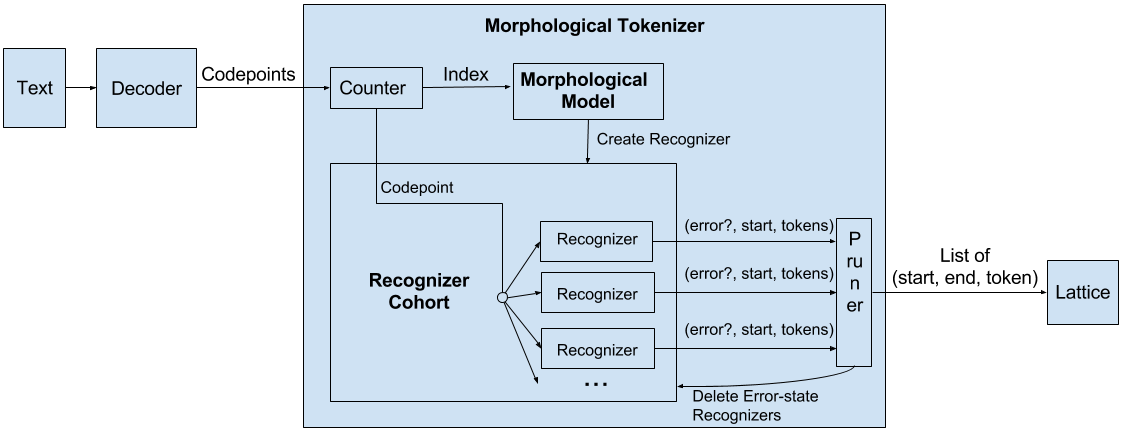
\includegraphics[width=\linewidth]{methodology/Morph}
	\caption{Morphological Tokenization}
	\label{morphdiagram}
\end{figure}

\subsection{Arabic}
Morphological tokenization of Arabic was accomplished using the MADAMIRA morphological analyzer\cite{pasha14}. MADAMIRA, unfortunately, does not expose an FSM network API, so it was necessary to collect complete candidate-token substrings to check all at once. Additionally, it does not provide any means of querying valid prefixes. In order to avoid quadratic or cubic runtime, which would make the experiment infeasible even on relatively short texts, extra rules were added to the interface connecting MADAMIRA to the generic tokenizer to reject strings satisfying certain conditions which I knew ahead of time could never result in valid prefixes. First, the interface would reject any string longer than 16 codepoints, as there were no tokens in the Arabic corpus greater than that length. Second, the interface would reject any string containing a whitespace character, since I knew ahead of time that the MADAMIRA lexicon did not contain any tokens containing whitespace characters.
In other respects, however, MADAMIRA is almost \textit{too} sophisticated to be effectively integrated into a tokenizer. In particular, MADAMIRA does not assume that the input will necessarily be a single word, and can analyze sentences with words in context; as a result, it does it's own word breaking (although the precise mechanism by which it does so is not described), and can return positive results for input containing more than one token. In order to account for this, MADAMIRA output was filtered to accept only those strings which MADAMIRA identified as containing exactly one "word". Additionally, MADAMIRA will "helpfully" ignore extraneous punctuation, leading it to produce valid analyses for words with, e.g., parentheses attached, as well as for the actual words themselves. I could find no principled way to avoid these spurious analyses, but, while they will result in reduced precision scores, they should not negatively affect recall.

MADAMIRA is accessed via an HTTP interface, which introduces significant I/O\footnote{Input/Output} overhead; in order to maximize CPU usage, the corpus was split into three parts, and three instances of the tokenizer were run simultaneously, accessing a single MADAMIRA server process.

\subsection{English}
Morphological tokenization of English was accomplished using the Englex morphological description of English\cite{antworthenglex} developed for PC-KIMMO\cite{koskenniemi84}. This model was run on a modified version of PyKIMMO\footnote{A Python implementation of the KIMMO two-level morphology algorithm.} known as Stream-KIMMO\cite{kearsley13}, which already has the appropriate FSM-like interface and required no adaptation. While the system runs in linear time, however, the original PyKIMMO implementation was highly inefficient, and introduced an enormous constant-factor slowdown, proportional to the size of the lexicon, due to simulating an FSM by dynamically calculating transitions and new states by iterating over the entire plain-text lexicon on every character. Re-implementing the core of PyKIMMO to construct a real FSM was not a viable option, but I was able to introduce several efficiency improvements which sped up the algorithm by approximately a factor of five; still, the relative slowness of this analyzer limited the quantity of text that could be processed from the OANC within a reasonable time frame. The English morphological experiment was thus terminated after approximately four days, at which time significantly more text had been processed than was available in the Korean corpus.

\subsection{Korean}
Morphological tokenization of Korean was accomplished using the KLEX morphological analyzer developed for the Xerox Finite-State Tools (XFST). KLEX was originally design to operate with input in either KSC-5601 or Unicode 1.0 encoding. In order to comply with modern versions of XFST, which only accept UTF-8 or Latin-1 encodings, and to enable it to work with the corpus which had been converted into UTF-8, it was necessary to modify the KLEX source code. Fortunately, KLEX had been designed to transliterate Hangul into a modified Yale romanization for internal processing and back again; thus, updating it for modern encodings was a simple matter of running a search-and-replace on the file containing Hangul-Yale equivalencies to replace the old Korean codepoints with modern Unicode 8.0 UTF-8 codepoints.
Python bindings for the XFST library do exist which are supposed to directly expose the underlying FSM, allowing linear-time traversal. These tools have, however, not been maintained, and I was unable to successfully install the software. Instead, it was necessary to make use of a simpler Python API exposing only the "apply up" and "apply down" functions of the morphological analyzer. As with MADAMIRA, it was thus necessary to introduce special-case rules which rejected any string longer than 22 codepoints (again based on the maximum-length token known to exist in the corpus), and to reject any string containing whitespace, again based on prior knowledge that the KLEX lexicon contained no tokens containing whitespace.
KLEX has the ability to recognize certain suffixes and clitics in isolation, if they are prefixed with the tag "\^DEP+" to indicate their status as bound (dependent) morphemes. Thus, in order to account for at least some possible variation in tokenization conventions, I ran two experiments with the morphological tokenizer on Korean: one which ignored dependents, and one which checked every possible token alone and with "\^DEP+" prefixed.

\subsection{Analyzer Coverage}
Since morphological tokenization depends on a morphological analyzer to identify lexical items and other valid tokens, the accuracy and recall of the morphological tokenizer in any particular language is dependent on the qualities of the analyzer available for that language. In particular, we can expect maximum accuracy and recall measurements when the definition of a 'token' used by the creator of a morphological analyzer is the same as the definition of a token used by the corpus annotator. Additionally, we can expect recall to be approximately bounded by the percentage of actual tokens in the corpus that are recognizable by the analyzer in isolation, with any missed tokens being restricted to those that are out-of-vocabulary for the analyzer.
In order to control for the quality of the analyzers used, coverage tests were run for each language to measure the fraction of tokens and types in the answer key that were recognizable by the analyzer for each language.

\subsection{Evaluation}
Morphological experiments were evaluated on recognition of starting boundaries, ending boundaries, total individual boundaries, and matched pairs. Precision, recall, F-score, and an adjusted recall (consisting of recall divided by analyzer token coverage) were calculated for each. Merging the starting and ending sets into total undifferentiated boundaries was done for easier comparison with statistical methods.
With no generic method of controlling for the effects of differing effective token definitions between corpora and morphological analyzers, I obtained qualitative results by manual inspection of the lists of missed tokens for each language.

\section{Statistical Tokenization}
In order to create a predictive model for statistical tokenization, mutual information (MI) scores were first compiled for every pair of codepoints present in each corpus. For this purpose, MI is given by the formula $\log_2(\frac{P(a,b)}{P(a)P(b)})$, where $a$ and $b$ are adjacent codepoints, $P(x)$ is the probability of encountering a given codepoint $x$ at any position, and $P(a,b)$ is the joint probability of encountering the pair of codepoints $a$ followed by $b$ at any given position. Word boundaries were then predicted by testing the MI score of each character pair in the corpora against a threshold value.
Two different methods of calculating thresholds were used in different experiments: gap threshold, and zero threshold. In the gap threshold method, the largest gap between MI scores for a given languages was identified, and a model was created which predicts a token boundary between every pair of codepoints whose mutual information score falls below that gap. This encodes the intuition that there may be a significant clustering of codepoint pairs that can occur across token boundaries vs. codepoint pairs that tend to occur within tokens, and was previously found to produce extremely high recall with reasonable accuracy on English data\cite{kearsley14}. In the zero threshold method, boundaries are predicted between every pair of codepoints whose MI score is less than or equal to 0, for all languages. This encodes the intuition that there may be a token boundary wherever the probability of encountering a codepoint in that position is less than the overall probability of encountering that codepoint in any position.
Contrary to Rytting's method\cite{rytting04}, 2004), MI scores are used to make token boundary predictions directly, rather than weighting them against a known prior probability of a particular character pair marking a token boundary as determined from training data. This simplification results in a completely unsupervised system, which makes it attractive for use in a hybrid system as it avoids increasing the amount of language-specific configuration needed beyond the dictionary or morphological model. Additionally, although in this case MI scores were calculated ahead of time to maximize performance, with either threshold-assignment method the model could be updated on-line, as in Brent's prior work\cite{brent99}, during real-time processing of a large input stream.
As in the morphological experiments, the output of each statistical experiment was saved to allow replaying the output for hybrid experiments. Since the statistical methods only identify single boundaries between tokens, rather than pairs bounding the start and end of a token, the saved output in this case consists of only a single list of possible boundary indices.

\begin{figure}[ht!]
	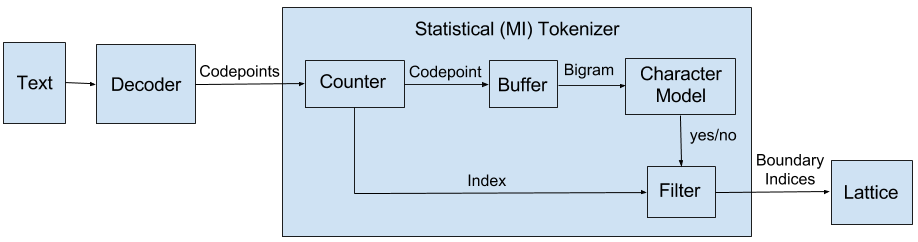
\includegraphics[width=\linewidth]{methodology/MI}
	\caption{Statistical Tokenization}
	\label{statdiagram}
\end{figure}

\subsection{Evaluation}
Like the morphological experiments, statistical experiments were evaluated on recognition of starting boundaries, ending boundaries, total individual boundaries, and matched pairs.
Since statistical predictions do not distinguish starting boundaries from ending boundaries, precision (the fraction of total predictions that are correct)  for starting and ending boundaries individually is skewed, as they were determined by the total number of correctly-predicted boundaries that are starting (or ending) boundaries over the total number of undifferentiated boundaries predicted. This makes comparisons with the precision and F-scores for other methods slightly suspect. Recall, however, could be calculated normally for start and ending boundary predictions, and all three measures were calculated normally for the total set of individual boundaries.
Token recall was calculated based on the number of (start, end) pairs in the answer key for which both starting and ending indices appeared in the statistical output. In place of precision for complete tokens, statistical results were also evaluated on what fraction of all codepoint boundaries were identified as possible token boundaries.

\section{Hybrid Tokenization}
I tested two methods of combining statistical and morphological methods to produce an improved hybrid tokenization system, which may be termed "filtering" and "filling". Each of these was run with the output of both zero-threshold and gap-threshold statistical experiments, for a total of four hybrid experiments.
The filtering method is an attempt to improve run-time efficiency and precision by only initiating a new recognizer to add to the active cohort in the morphological tokenizer at indices where the statistical model indicates a token boundary is likely. This was simulated by constructing a new stream of (start, end) index pairs from stored morphological output including only those pairs in which the start index exists in the stored statistical data.
The filling method is an attempt to improve recall and address the limitations of lexical-access based tokenization methods (including morphological tokenizers) by using statistical predictions to fill in gaps of unanalyzed codepoints between tokens identified by the morphological model. This was simulated by identifying spans of codepoints not covered by any (start, end) pair in the morphological output, and filling them in with all (start, end) pairs that could be constructed from the predictions of the statistical models over those spans.

\begin{figure}[ht!]
	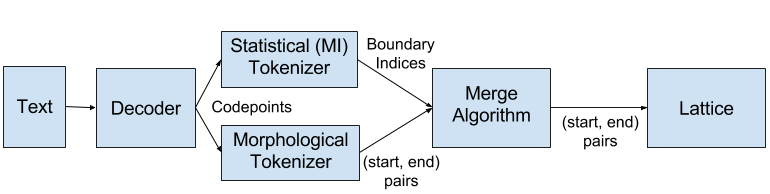
\includegraphics[width=\linewidth]{methodology/Hybrid}
	\caption{Hybrid Tokenization}
	\label{hybriddiagram}
\end{figure}

\subsection{Evaluation}
As in the morphological experiments, precision, recall, and F-score were calculated for starting boundaries, ending boundaries, total individual boundaries, and matched pairs for all hybrid experiments. Additionally, a reduction factor was calculated for the filter experiments, consisting of the total number of token boundaries output by the filtering algorithm divided by the number of boundaries present in the raw morphological output.